
A test version of the predictive event processing network was created with Java programming language. Java was chosen because of several reasons:
\begin{itemize}
\item{Java is the main development language of MMEA platform}
\item{Esper CEP Engine provides easy-to-use API for Java}
\item{Test data is available via a Java library}
\item{The performance of Java is sufficient}
\end{itemize}

Unlike the MMEA platform that uses PostgreSQL and Amazon S3 as database solutions, I have chosen MySQL as my development database because I am more familiar with it. I use an ORM (Object-relational mapping) layer called Hibernate between my program and the database. Thus, using a different database solution is only a matter of changing the database adapter from MySQL to something else in the Hibernate configuration file.

The goal of this chapter is to present a framework for integrating a predictive component alongside with a Event Processing Network. The approach is quite technical meaning that anyone with adequate skills in Java and Esper could replicate the system and improve it with their own expertise.

\subsection{Data Structures}
The test data is mapped into four Java classes that directly correspond to tables in my own MySQL database. This mapping is done with Hibernate library, which allows the programmer to annotate, that is, add table specifications Java classes. Then, Hibernate creates the database schema using these annotations. In the following I will describe these four classes in a compact form stating only the name of the class and parameter types and names. 

First class represents the house we are dealing with:
\begin{Verbatim}[xleftmargin=1.5em]
public class House {
	int houseId;
	String name;
	Map<Integer, Sensor> sensors;
	Set<MeasurementUnit> units;
},
\end{Verbatim}
where, the parameter \emph{sensors} is a map from sensor IDs to sensor objects and the parameter \emph{units} contains all the measurement events from that house.

The second class represents a single sensor:
\begin{Verbatim}[xleftmargin=1.5em]
public class Sensor {
	House house;
	int sensorId;
	String name;
}
\end{Verbatim}

The third class represents a single measurement event which, in turn, may contain multiple measurement values from different sensors:
\begin{Verbatim}[xleftmargin=1.5em]
public class MeasurementUnit implements TimedEvent {
	House house;
	Date timestamp;
	Set<MeasurementValue> values;
}
\end{Verbatim}

The last class represents a single measurement value:

\begin{Verbatim}[xleftmargin=1.5em]
public class MeasurementValue {
	Sensor sensor;
	MeasurementUnit measurementUnit;
	double value;
}
\end{Verbatim}

As can be seen, \emph{MeasurementUnit} class implements an interface called \emph{TimedEvent} which is a common interface for all events in this thesis. It requires the class to have a timestamp property that can be used to mark the occurrence of an event in the time space. Objects from the class \emph{MeasurementUnit} are the most important ones because the event source emits them to the CEP engine. The processing of these events is described in the following chapter.



\subsection{Predictive Event Processing Network}
The Predictive Event Processing Network (PEPN) is a separate network as described in Chapter 3.2. In this thesis I have made the separation so clear that the two networks even have their own Esper engines. In some publications (e.g. \cite{Fulop12}) the PEPN just integrates into the EPN's engine but in this thesis' approach some Event Processing Agents (EPAs) connect to both networks and transfer data between them. 

The structure of the Event Processing Network (EPN) defines which Complex Events the system captures and it depends on the phenomenon in question. However, the structure of the PEPN is completely independent of the EPN meaning that the framework presented here should, in theory, work for each Complex Event type that is predictable with the predictive models used here. The phenomenon-specific EPNs (and its EPAs) will be defined in experimental design chapter. The framework for PEPN is presented in Figure~\ref{fig:pepn}.

\begin{sidewaysfigure}[here]
\centering
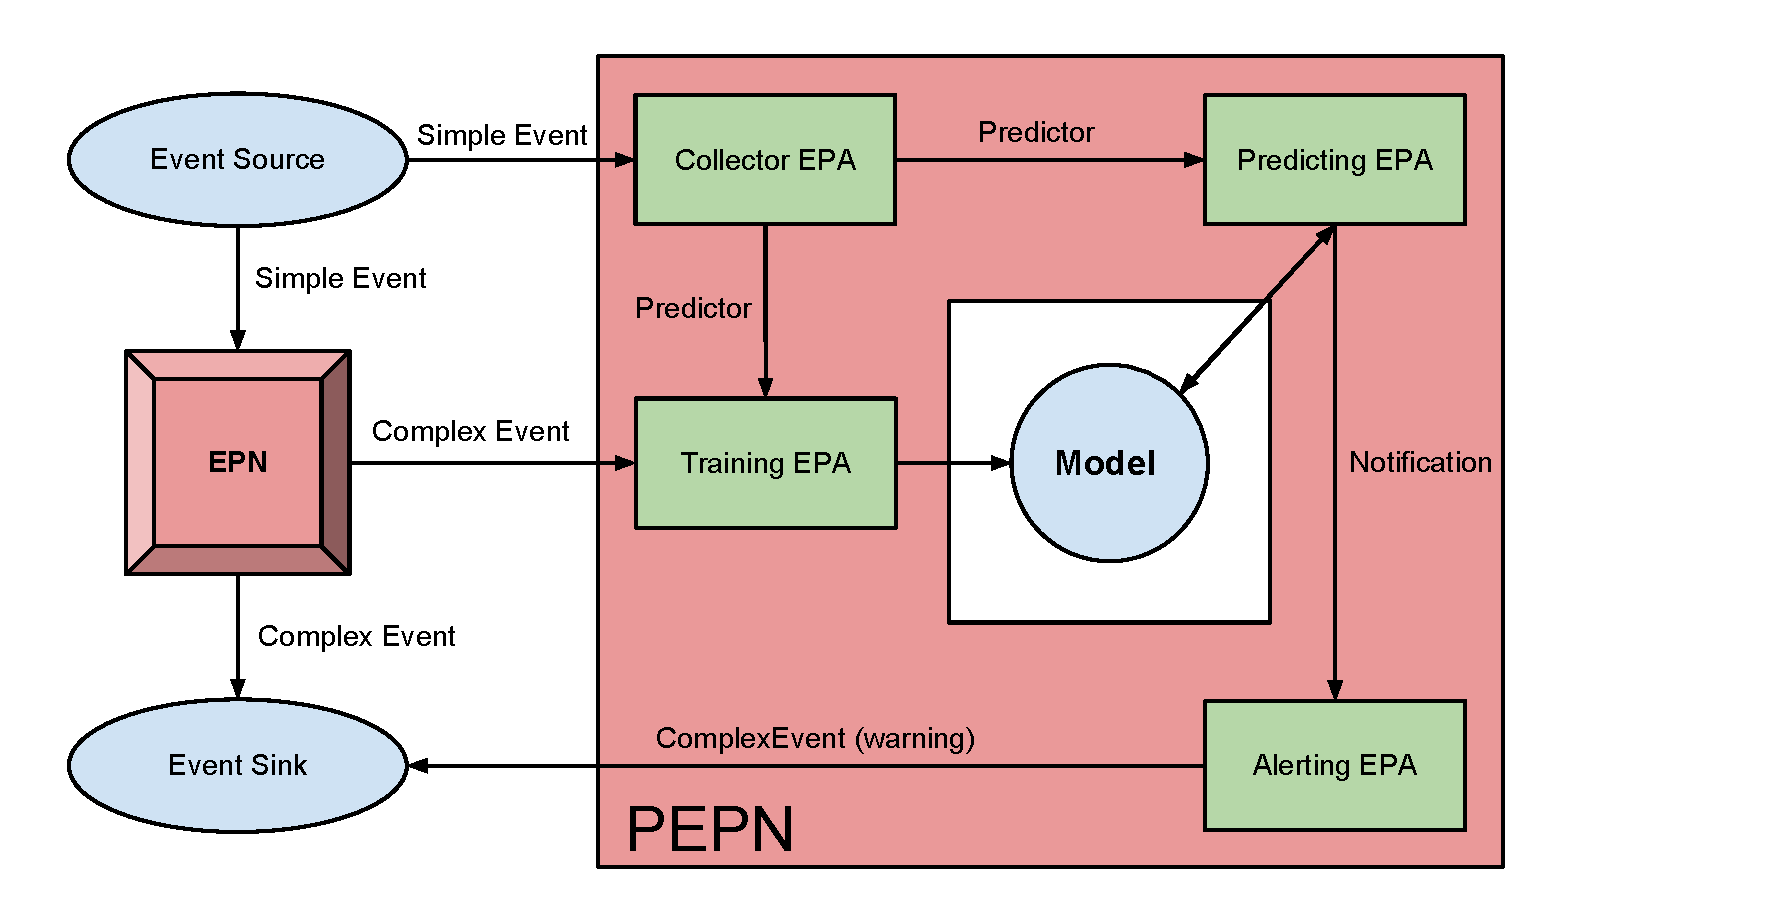
\includegraphics[scale=0.7]{images/epn.pdf}
\caption{Event Processing Network (EPN) and Predictive Event Processing Network.}
\label{fig:pepn}
\end{sidewaysfigure}


On the left side of the figure there is the EPN that attaches to the event sources, processes the data and outputs a Primary Complex Event (PCE) to the event sink. In this concept we don't place any restrictions for neither the format of input data nor the structure of the data processing. However, the output of the EPN must be unique, that is, only one type of output is allowed. Thus, the output can be formalized as the following Java class
\begin{Verbatim}[xleftmargin=1.5em]
public class ComplexEvent {
	Date timestamp;
	String message;
},
\end{Verbatim}
where the timestamp marks the time when the complex event takes place and the message contains relevant information about the event type that can be shown to the user when the event happens. 

In Esper an event listener specifies an EPL and implements the interface
\begin{Verbatim}[xleftmargin=1.5em]
public interface UpdateListener {
	public void update(EventBean[] newEvents, EventBean[] oldEvents);
}
\end{Verbatim}

When the EPL is triggered, the \emph{update} method is called and the events entering the window are given in \emph{newEvents} array while the events leaving the window can be found from \emph{oldEvents}. \cite{EsperReference} In this thesis, an Event Processing Agent (EPA) is required to provide an EPL clause and to implement the interface above.


The Predictive Event Processing Network (PEPN) has four different Event EPAs that collect and preprocess the incoming data. 

\emph{CollectorEpa} listens to EPN's event sources and collects predictor vectors for training and predicting phases. Its EPL is of the form
\begin{Verbatim}[xleftmargin=1.5em]
SELECT 
	value('<sensorId>').value as value, 
	time 
FROM 
	MeasurementUnit.win:time(<windowLength>)
OUTPUT SNAPSHOT
	every <windowDifference>
\end{Verbatim} 

Here the first select item uses \emph{MeasurementUnit}'s getter for measurement values and then uses its getter for value. The clause defines a sliding window whose length is given as a parameter \emph{windowLength} for the EPL. The last part, \emph{output snapshot every windowDifference}, triggers the \emph{update} method with the given time interval. Then, Esper's pull API allows us to iterate through the window's contents. \cite{EsperReference} This EPL creates the predictor vectors that are then consumed by other EPAs.

Next, as can been from Figure~\ref{fig:pepn}, \emph{TrainingEpa} and \emph{PredictingEpa} use the predictors emitted by \emph{CollectorEpa} as their input. In this case, the predictors are instances of the class \emph{MeasurementVector}, which is of the following form
\begin{Verbatim}[xleftmargin=1.5em]
public class MeasurementVector implements TimedEvent, LabeledSample {
	Date timestamp;
	Date endTimestamp;
	List<Double> values;
	Label label;
},
\end{Verbatim}
where values list contains the measurement values between \emph{timestamp} and \emph{endTimestamp}. \emph{MeasurementVector} is a time series which we are trying to classify. It implements the interface \emph{LabeledSample} which requires it to have a \emph{Label} property. The \emph{TrainingEpa} listens also to the EPN's \emph{ComplexEvent}s and its EPL is as follows
\begin{Verbatim}[xleftmargin=1.5em]
SELECT predictor.*
	FROM pattern[
		every predictor=MeasurementVector 
		-> (timer:interval(<waitingTime>) 
		-> (timer:interval(<eventTime>) and <Negation>c=ComplexEvent))
	],
\end{Verbatim} 
which needs a bit clarification. The pattern in the EPL first looks for a \emph{MeasurementVector} event from \emph{CollectorEPA}. The \emph{every} keyword initiates this lookup on each event. When an event is found, the first timer waits an interval of length \emph{waitingTime}. Then, the second interval looks for an interval of length \emph{eventTime} during which a \emph{ComplexEvent} is found. The variable \emph{Negation} is either empty or ``not '', which allows us to detect both positive and negative instances. For this purpose, we can define two \emph{TrainingEPA}s: one for positive instances with \emph{Negation} being empty and one for negative instances with \emph{Negation} set to ``not ''.

Now the \emph{TrainingEPA} collects the predictors but the next step is to decide when to perform the actual training process. For this purpose a \emph{TrainingInvokerEPA}, which is not shown in the pictures as it ``lives'' inside the \emph{TrainingEPA}. It declares an EPL of the form

\begin{Verbatim}[xleftmargin=1.5em]
SELECT 
	* 
FROM 
	pattern[every timer:interval(<trainingInterval>)],
\end{Verbatim} 
which is triggered automatically based on the time variable \emph{trainingInterval}. Then, the \emph{update} is called and it executes the training of the model.

Like the \emph{TrainingEpa}s, \emph{Predictor}EPA is fed with predictors (\emph{MeasurementVectors}) as shown in Figure~\ref{fig:pepn}. Both \emph{TrainingEPA}s and \emph{PredictorEPA} communicate directly with a specific model class that extends an abstract \emph{Model} class. Sub-classes of Model implement a certain model, in this case either a DTW and kNN-based one or a Wavelet and SVM-based one. The Model collects labeled predictors from \emph{TrainingEPA}s until its \emph{train()} method is called.

The \emph{PredictorEpa}, in turn, calls the Model's classify(\emph{MeasurementVector})-method, which returns the label for the given predictor. If the instance is classified as positive, a notification event is sent to the PEPN, which is then captured by \emph{AlertingEPA}. Then, the \emph{AlertingEPA} builds a \emph{ComplexEvent} and outputs it to the original EPN. In this way, the PEPN creates a warning for the EPN.


\subsection{Data Flow and Performance Tuning}
The event source reads a block of data from the database and sends it to both EPN and PEPN as can be seen in Figure~\ref{fig:pepn}. Then, the event processing networks process the data with their own EPAs. Without giving any thought to concurrency, this approach faces the problem of blocking as the event source does not start reading new data until the processing of old data is finished. 

To solve this problem we use threads that are kind of lightweight processes. \cite{Java} Unlike actual processes, threads share the same memory space and are actually contained within one process. On a single-core processor the operating system can use time slicing feature to allow threads to execute code almost concurrently. On a multi-core processor the system's capability for concurrent processes enhances significantly.

Our system has four threads: main thread, event source thread, EPN thread and PEPN thread. The last three threads are initialized and started from the main thread. To exchange data between two threads we need a data structure that supports concurrent processing. The data structure should be some kind of queue as the event source fills it with data and the two networks read from it. The Java programming language offers several implementations for concurrent queues. A suitable choice is \emph{LinkedBlockingQueue}, a First-In-First-Out (FIFO) queue, which offers the following methods \cite{Java}
\begin{description}
\item[void put(Object)]{Inserts the specified element into this queue, waiting if necessary for space to become available.}
\item[void take()]{Retrieves and removes the head of this queue, waiting if necessary until an element becomes available.}
\end{description}

In our system there are two of these queues: one between event source and EPN and one between event source and PEPN. Now the event source can read a batch of data from the database and call \emph{put(e)} for each element. Then, both networks, being in an infinite loop calling \emph{take()}, start processing data as soon as it becomes available.




\subsection{Machine Learning Libraries}
In this thesis I use two ready-made machine learning libraries: Java Machine Learning Library (Java-ML) \cite{javaml} and Weka 3: Data Mining Software in Java \cite{weka}. This approach allows me to concentrate not on the implementation of the algorithms but on the proper use of the methods. More importantly, the algorithms used in the libraries have already been optimized and tested properly by machine learning experts.

Java-ML contains an implementations for Dynamic Time Warping (DTW) and k-Nearest Neighbor (kNN) algorithms. Together with Java-ML's \emph{CrossValidation} class, it is fairly easy to choose optimal parameter values. This algorithm, however, lacks the possibility of receiving intermediate results. For this reason I created an implementation by following the pseudo-code from section 3.6.1.

For a given set of parameters, the cross validation algorithm returns an instance of the class \emph{PerformanceMeasure}, which contains the variables TP, FP, TN and FN. From these I calculate the value for the $AC_d$ as described in (109)-(116). Then, the set of parameters with the lowest $AC_d$ is chosen.

Java-ML has a wrapper for LibSVM which is an efficient Support Vector Machine library \cite{libsvm}. The interface provides Java classes that call the fast underlying C implementations. LibSVM comes with a class called \emph{GridSearch}, which performs the grid search for parameters $C$ and $\gamma$ as described in Chapter 3.5.7. Again, I implemented the grid search in order to receive intermediate results.

In this thesis the Weka library is used to perform the wavelet transform and it supports the Discrete Haar Wavelet Transform. The conversion between Weka and Java-ML data formats is easy as their \emph{Instance} classes provide getter and setter method for plain double arrays that contain the vector data.





